\documentclass{article}

\usepackage{graphicx}
\usepackage{amsmath}
\usepackage{microtype}
\usepackage{tikz}
\usetikzlibrary{decorations.pathreplacing}
\usepackage{caption}
\captionsetup{width=0.95\linewidth}

% Avoid tiny overfull boxes from long lines
\setlength{\emergencystretch}{5em}
\setlength{\hfuzz}{5pt}
\hbadness=10000

\title{Temporal Coherence in Long-Horizon, Intermittently Connected Sensor Systems}
\author{}
\date{}

\newcommand{\conceptual}{\textit{(conceptual illustration)}}

\begin{document}
\sloppy % reduce overfull boxes from long lines/nodes
\maketitle

\begin{abstract}
Long-horizon sensing systems operating under intermittent connectivity exhibit a characteristic failure mode: time becomes non-queryable (in the sense that basic provenance and causal queries cannot be answered reliably at the time operational decisions were made). Clock drift, buffering, and delayed uplink cause event time, record time, and ingest time to collapse into a single timestamp, destroying causal reasoning, undermining auditability, and reducing fleet-level value by forcing operators to revert to conservative or manual decision-making. This note describes the failure mode, explains why it becomes most visible in unmanned and remote systems, and proposes a minimal representation of time that preserves temporal coherence under intermittency, without requiring continuous synchronisation or retrospective revision.
\end{abstract}

\section{Introduction}

Modern sensing deployments increasingly rely on unmanned, remote, and power-constrained platforms operating for extended periods without continuous connectivity. Examples include seabed observatories, autonomous surface and subsurface vehicles, polar monitoring stations, and remote environmental sensor networks. In these settings, sensors must operate autonomously for long durations, often with limited opportunities for communication or maintenance.

While sensor fidelity, storage capacity, and communications bandwidth have improved significantly, system-level temporal coherence has not kept pace. In many long-horizon deployments, the first thing to degrade is not sensing or transport, but temporal coherence. Data continues to arrive and deployments appear operational, yet the ability to reason about sequence, simultaneity, and causality quietly degrades.

This degradation is rarely treated as a first-order systems problem. Instead, it is often addressed implicitly, through ad hoc timestamp correction or manual interpretation. The result is data that appears precise but is increasingly difficult to trust as deployments scale in duration, autonomy, and complexity.

This failure mode is architectural rather than algorithmic, and therefore persists across vendor changes, firmware updates, and platform refreshes. Improvements in sensing accuracy or bandwidth alone do not resolve the problem, and may in fact amplify downstream confusion. As a result, programmes may appear to modernise while retaining the same latent decision risk. It does not arise from inadequate sensing or transport, but from the implicit assumption that time can be collapsed into a single authoritative scalar during ingestion. Specifically, systems tend to collapse event time, record time, and ingest time into a single scalar timestamp without preserving uncertainty or provenance. The consequences surface downstream, at the level of analysis, assurance, and decision-making. As such, temporal coherence must be treated as a system property that spans sensing, buffering, transport, and ingest, rather than a local implementation detail.

\section{From Seabed to Screen}

Consider a distributed maritime sensing deployment comprising seabed nodes, autonomous surface or sub-surface vehicles, and intermittent satellite uplink to shore-based analysis. Individual platforms operate autonomously for extended periods, resynchronising clocks only opportunistically when surfaced, serviced, or recovered. In many cases, such recovery occurs long after the operational decisions that depended on the data. Observations may traverse multiple buffering stages before ingestion, with delays spanning minutes to weeks. In such deployments, temporal coherence can degrade even when sensing and transport remain nominally operational.

A typical long-horizon sensing deployment spans multiple temporal domains:

\begin{itemize}
  \item Sensor-local clocks operating under power and thermal constraints
  \item Intermediate gateways such as seafloor nodes, buoys, or vehicles
  \item Transport layers including acoustic links, satellite uplinks, fibre connections, or physical retrieval
  \item Ingest systems that assign arrival-time timestamps
  \item Analytical systems that assume a single global timeline
\end{itemize}

Each layer maintains its own notion of time, often with different accuracy, stability, and update frequency. In many systems, these distinct temporal domains are collapsed implicitly during ingestion, producing a single timestamp that is treated as authoritative. This collapse typically occurs by default rather than by deliberate design, as no single team owns temporal semantics end-to-end. Temporal semantics emerge implicitly from the interaction of independently designed components, rather than being specified or enforced explicitly.

This collapse is convenient but misleading. The resulting timestamp is neither purely an event time nor a record time, but a hybrid whose meaning depends on undocumented assumptions about buffering, drift, and correction. Outside its immediate context, the timestamp no longer supports reliable reasoning.

\section{Failure Mode}

\subsection{Clock Drift at the Edge}

Edge sensors frequently rely on inexpensive oscillators that drift seconds to minutes over weeks or months. Continuous synchronisation (e.g., GNSS) is often unavailable due to depth, power constraints, or environmental conditions. As a result, sensors may only resynchronise when surfaced, serviced, or physically recovered.

When drift is corrected, it is often applied as a step adjustment, retroactively shifting all prior timestamps long after operational decisions have already been taken. At that point, the system’s historical state no longer reflects the information actually available when those decisions were made. The uncertainty introduced by drift is rarely preserved or propagated, and downstream systems are not informed that historical timestamps have been modified.

\subsection{Asymmetric Buffering and Burst Upload}

Intermittent connectivity forces sensors and gateways to buffer data locally and transmit it in bursts. Data arrival time at the ingest system may lag event time by minutes, hours, or weeks. Buffering can also introduce reordering, partial uploads, or duplication.

Despite this, ingest systems often conflate arrival time with event time, either by overwriting timestamps or by implicitly privileging the time of receipt. This erases information about when observations actually occurred.

\subsection{Arrival Time Masquerading as Event Time}

Dashboards and alerting systems often assume that timestamps represent the moment an event occurred. When arrival time is substituted for event time, correlations appear that are artefacts of transport rather than reality. Spurious simultaneity and false causality become difficult to detect.

The system continues to function, but its outputs no longer correspond cleanly to the physical world it is meant to observe.

Operators often compensate informally by mentally re-timestamping data or discounting automation, masking the issue until scale or autonomy removes the human from the loop.

\subsection{Loss of Auditability}

Once timestamps are normalised or overwritten without provenance, it becomes impossible to reconstruct what the system knew at a given moment. Questions such as ``What information was available when this decision was made?'' or ``Which observations could have influenced this alert?'' cannot be answered reliably.

Each subsequent normalisation or overwrite further weakens the ability to reconstruct ordering, provenance, and system state at the time of decision. This loss of auditability is cumulative and often invisible until trust has already eroded.

Once temporal provenance has been overwritten or discarded, it cannot be reconstructed after the fact; no amount of downstream sophistication can recover it.

From an assurance perspective, this undermines the ability to defend decisions after the fact. Without preserved temporal provenance, it is not possible to demonstrate what information was available at the time a decision was taken, nor to bound which observations could have influenced it. This complicates safety cases, incident investigation, and regulatory or legal scrutiny. The resulting loss of trust is systemic rather than sensor-specific.

\section{Reframing Time}

Rather than treating time as a scalar, we treat it as a bounded estimate with provenance. Event time is separated explicitly from record time and ingest time, and uncertainty is represented as a first-class property of each observation.

This reframing mirrors informal human reasoning about delayed observations, but the contribution here is not cognitive—it is architectural. Operators naturally discount older or less certain data and reason in terms of windows rather than points. This observation is used only as an analogy for informal practice; the goal is to formalise temporal uncertainty so systems can behave consistently under intermittency. The contribution here is to render this reasoning explicit, machine-readable, and enforceable in software.

\section{A Minimal Model}

\subsection{Event Representation}

Each observation carries:

\begin{itemize}
  \item An estimated event time
  \item A temporal uncertainty bound
  \item Clock provenance (e.g., sensor, gateway, external reference, inferred)
  \item Time since last synchronisation
\end{itemize}

Formally, event time is represented as an interval rather than a point:
\[
  t_{\text{event}} \in [t - \epsilon,\, t + \epsilon]
\]
where $\epsilon$ is a conservative upper bound on accumulated temporal uncertainty due to drift and transport, which grows with time since the last trusted anchor.

Responsibility for maintaining conservative and honest uncertainty bounds must be explicit, as overly optimistic bounds reintroduce false precision; overly conservative bounds reduce utility but preserve correctness.

\subsection{Temporal Ordering}

Event ordering is defined only when justified by uncertainty bounds. Given two events $A$ and $B$ with intervals $[A^{-}, A^{+}]$ and $[B^{-}, B^{+}]$, we say that $A$ precedes $B$ if and only if:
\[
  A^{+} < B^{-}
\]

If the intervals overlap, no ordering is asserted. In many deployed pipelines, interval information is discarded at ingestion, permanently eliminating safe partial ordering even when the underlying system uncertainty would have permitted it. This preserves causal ambiguity rather than forcing a false total order.

\subsection{Invariants}

The system enforces a small set of invariants:

\begin{itemize}
  \item Event time is never overwritten
  \item Uncertainty never shrinks without a new temporal anchor
  \item Corrections are additive and auditable, not destructive
\end{itemize}

These invariants constrain behaviour without prescribing a specific synchronisation mechanism or transport architecture.

These invariants are compatible with incremental adoption. Systems may coexist with legacy timestamped data, and the model does not require changes to sensing hardware or transport layers. Temporal coherence can therefore be introduced selectively, at points of ingestion or analysis, without wholesale architectural replacement.

\section{Relation to Prior Approaches}

Related problems have been addressed in adjacent domains, including clock synchronisation protocols, event-time processing in data streams, and causal ordering in distributed systems. These approaches typically assume frequent communication, stable clocks, or the ability to overwrite timestamps as improved information becomes available. Examples include event-time semantics in stream processing, clock synchronisation in time-sensitive networking, and partial orders in distributed systems; each addresses a facet of the problem but typically assumes stable connectivity or revisable history.

Long-horizon, intermittently connected sensing systems violate these assumptions. Synchronisation opportunities are sparse, drift accumulates continuously, and historical data cannot be revised without destroying auditability. As a result, existing approaches do not preserve temporal coherence under the conditions considered here.

In operational and regulated settings, revising historical time undermines the ability to defend decisions based on contemporaneous knowledge, decisions must be defensible based on the information available at the time, not on retrospectively revised history.

This work reframes time not as a synchronisation problem, but as an architectural property that must persist across sensing, buffering, and delayed ingestion.

\section{Operational and Assurance Implications}

\subsection{Queryable Time}

Once time is represented explicitly, systems can answer questions that are otherwise ill-defined:

\begin{itemize}
  \item What was known at a given time?
  \item Which correlations are temporally plausible?
  \item Which observations could have influenced a decision?
  \item Whether a different action would have been reasonable given the information available at the time?
\end{itemize}

Time becomes queryable rather than assumed.

\subsection{Fleet-Level Value}

When temporal uncertainty is bounded and explicit, data from multiple platforms can be correlated without false precision. Operationally, this manifests in tighter operating envelopes, fewer manual overrides, and increased confidence in automated recommendations. The analytical value of a fleet increases materially once coherence is preserved, because cross-platform reasoning no longer relies on brittle assumptions about simultaneity.

\subsection{Why Autonomy Makes the Problem Observable}

When humans are present on platforms, continuity often lives in people. Operators implicitly reconcile delays, drift, and context. As platforms become unmanned, that continuity has nowhere to live unless it is encoded in the system itself.

Autonomy does not create the temporal problem; it makes it observable.

For long-horizon sensing programmes, this reframing enables fleets to scale in duration, autonomy, and heterogeneity without a corresponding loss of trust or auditability.

These effects are most pronounced in high-latitude and polar deployments, where thermal drift, sparse synchronisation opportunities, regulatory scrutiny, and delayed recovery compound temporal incoherence.

\section{Conclusion}

Temporal coherence is a prerequisite for trustworthy long-horizon sensing. Systems that preserve temporal provenance retain analytical and operational value under intermittency; systems that do not instead accumulate unbounded ambiguity in ordering, provenance, and auditability. Temporal coherence is not a property of clocks or networks, but of system architecture. By preserving temporal provenance, architectures retain the ability to explain and defend decisions long after deployment, even under prolonged intermittency.

\begin{figure}[ht]
\centering
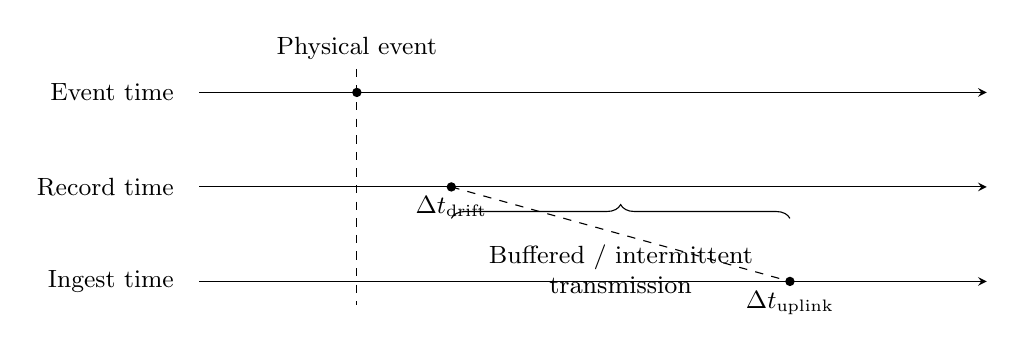
\begin{tikzpicture}[
  x=1cm,
  y=1cm,
  >=stealth,
  every node/.style={font=\small},
  timeline/.style={->},
  point/.style={circle,fill,inner sep=1.2pt}
]
  % Coordinates
  \def\xEvent{2}
  \def\xRecord{3.2}
  \def\xIngest{7.5}
  \def\xEnd{10}

  \coordinate (E) at (\xEvent,0);
  \coordinate (R) at (\xRecord,-1.2);
  \coordinate (I) at (\xIngest,-2.4);

  % Row labels
  \node[anchor=east] at (-0.2, 0) {Event time};
  \node[anchor=east] at (-0.2, -1.2) {Record time};
  \node[anchor=east] at (-0.2, -2.4) {Ingest time};

  % Timelines
  \draw[timeline] (0,0) -- (\xEnd,0);
  \draw[timeline] (0,-1.2) -- (\xEnd,-1.2);
  \draw[timeline] (0,-2.4) -- (\xEnd,-2.4);

  % Physical event marker
  \draw[dashed] (\xEvent,0.3) -- (\xEvent,-2.7);
  \node[anchor=south] at (\xEvent,0.3) {Physical event};

  % Points
  \node[point] at (E) {};
  \node[point] at (R) {};
  \node[point] at (I) {};

  % Drift and uplink offsets
  \draw[dashed] (\xEvent,-1.2) -- (R);
  \node[anchor=north] at (R) {$\Delta t_{\text{drift}}$};

  \draw[dashed] (R) -- (I);
  \node[anchor=north] at (I) {$\Delta t_{\text{uplink}}$};

  % Buffer annotation
  \draw[decorate,decoration={brace,amplitude=5pt}]
    (\xRecord,-1.6) -- (\xIngest,-1.6)
    node[midway,below=6pt,align=center,text width=4cm]{Buffered / intermittent\\ transmission};
\end{tikzpicture}
\caption{Temporal domains in a typical long-horizon sensing stack. A single physical event maps to divergent timestamps under clock drift and delayed uplink. Event time, record time, and ingest time must be represented explicitly to preserve causal coherence.}
\end{figure}

\begin{figure}[ht]
\centering
\resizebox{\linewidth}{!}{
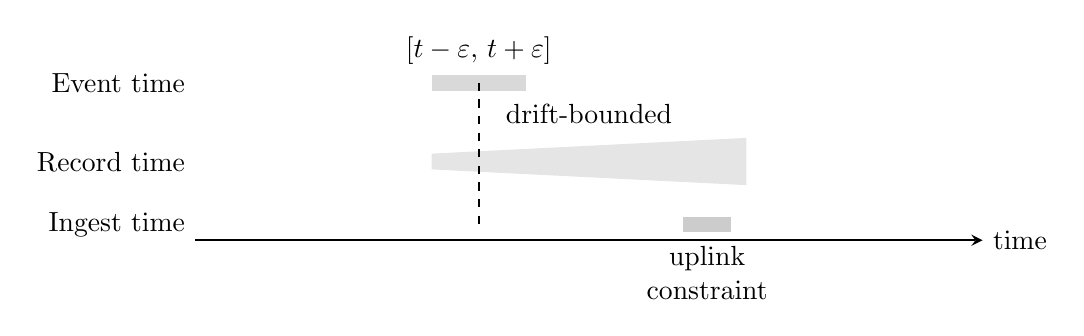
\begin{tikzpicture}[>=stealth, thick]

% Time axis
\draw[->] (0,0) -- (10,0) node[right] {time};

% Labels
\node[left] at (0,2) {Event time};
\node[left] at (0,1) {Record time};
\node[left] at (0,0.2) {Ingest time};

% Event time uncertainty band
\fill[gray!30] (3,1.9) rectangle (4.2,2.1);
\node[above] at (3.6,2.1) {$[t-\varepsilon,\, t+\varepsilon]$};

% Record time drift band
\fill[gray!20] (3,0.9) -- (3,1.1) -- (7,1.3) -- (7,0.7) -- cycle;
\node[above] at (5,1.35) {drift-bounded};

% Ingest time contraction
\fill[gray!40] (6.2,0.1) rectangle (6.8,0.3);
\node[below,align=center] at (6.5,0.05) {uplink\\constraint};

% Vertical projection
\draw[dashed] (3.6,2) -- (3.6,0.2);

\end{tikzpicture}
}
\caption{Temporal coherence with propagated uncertainty. Event time is represented as an interval whose uncertainty evolves across sensing, buffering, and uplink rather than collapsing into a single timestamp.}
\end{figure}

\begin{figure}[ht]
\centering
\resizebox{0.9\linewidth}{!}{%
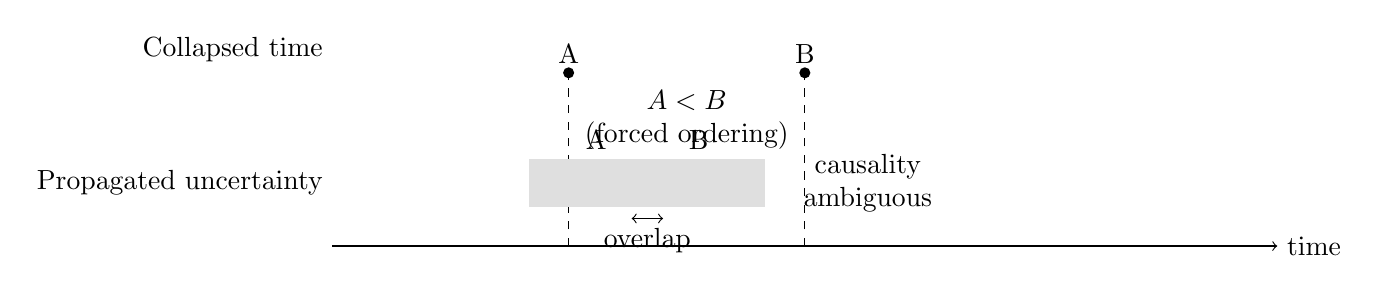
\begin{tikzpicture}[x=1cm,y=1cm]

% Time axis
\draw[->] (0,0) -- (12,0) node[right]{time};

% Labels
\node[anchor=east] at (0,2.5) {Collapsed time};
\node[anchor=east] at (0,0.8) {Propagated uncertainty};

% --- Collapsed representation ---
% Event A
\draw[dashed] (3,0) -- (3,2.2);
\fill (3,2.2) circle (2pt);
\node[above] at (3,2.2) {A};

% Event B
\draw[dashed] (6,0) -- (6,2.2);
\fill (6,2.2) circle (2pt);
\node[above] at (6,2.2) {B};

\node[align=center] at (4.5,1.6) {$A < B$\\(forced ordering)};

% --- Interval representation ---
% Event A interval
\draw[fill=gray!25,draw=none] (2.5,0.5) rectangle (4.2,1.1);
\node[above] at (3.35,1.1) {A};

% Event B interval
\draw[fill=gray!25,draw=none] (3.8,0.5) rectangle (5.5,1.1);
\node[above] at (4.65,1.1) {B};

% Overlap annotation
\draw[<->] (3.8,0.35) -- (4.2,0.35);
\node[below] at (4.0,0.35) {overlap};

\node[align=center] at (6.8,0.8) {causality\\ambiguous};

\end{tikzpicture}
}
\caption{Temporal causality under collapsed versus propagated time. When timestamps are collapsed to points (top), events appear totally ordered even when that ordering is not justified; when uncertainty is propagated (bottom), overlapping event intervals make causal ambiguity explicit and queryable.}
\end{figure}

\begin{figure}[ht]
\centering
\scalebox{0.65}{%
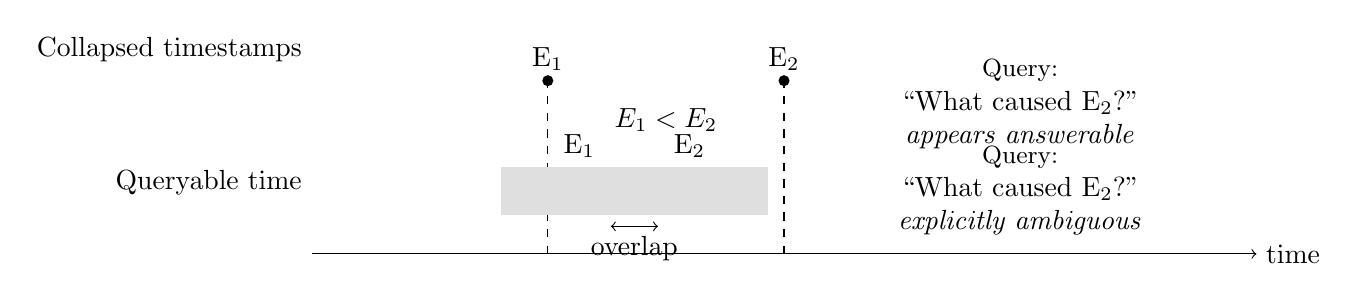
\begin{tikzpicture}[x=1cm,y=1cm]

% Time axis
\draw[->] (0,0) -- (12,0) node[right]{time};

% Labels
\node[anchor=east] at (0,2.6) {Collapsed timestamps};
\node[anchor=east] at (0,0.9) {Queryable time};

% ---- Collapsed case ----
% Events
\draw[dashed] (3,0) -- (3,2.2);
\fill (3,2.2) circle (2pt);
\node[above] at (3,2.2) {E$_1$};

\draw[dashed] (6,0) -- (6,2.2);
\fill (6,2.2) circle (2pt);
\node[above] at (6,2.2) {E$_2$};

% Forced ordering
\node at (4.5,1.7) {$E_1 < E_2$};

% Query annotation
\node[align=center] at (9,1.9)
  {\small Query:\\``What caused E$_2$?''\\\textit{appears answerable}};

% ---- Queryable case ----
% Event intervals
\draw[fill=gray!25,draw=none] (2.4,0.5) rectangle (4.4,1.1);
\node[above] at (3.4,1.1) {E$_1$};

\draw[fill=gray!25,draw=none] (3.8,0.5) rectangle (5.8,1.1);
\node[above] at (4.8,1.1) {E$_2$};

% Overlap marker
\draw[<->] (3.8,0.35) -- (4.4,0.35);
\node[below] at (4.1,0.35) {overlap};

% Query annotation
\node[align=center] at (9,0.8)
  {\small Query:\\``What caused E$_2$?''\\\textit{explicitly ambiguous}};

\end{tikzpicture}
}
\caption{Timestamp collapse versus queryable time. \conceptual\; When timestamps are collapsed to points (top), systems enforce a total ordering that makes causal queries appear answerable even when that ordering is unjustified; when temporal uncertainty is propagated (bottom), overlapping event intervals expose ambiguity, making causal queries explicit rather than silently wrong.}
\end{figure}

\begin{figure}[ht]
\centering
\scalebox{0.65}{%
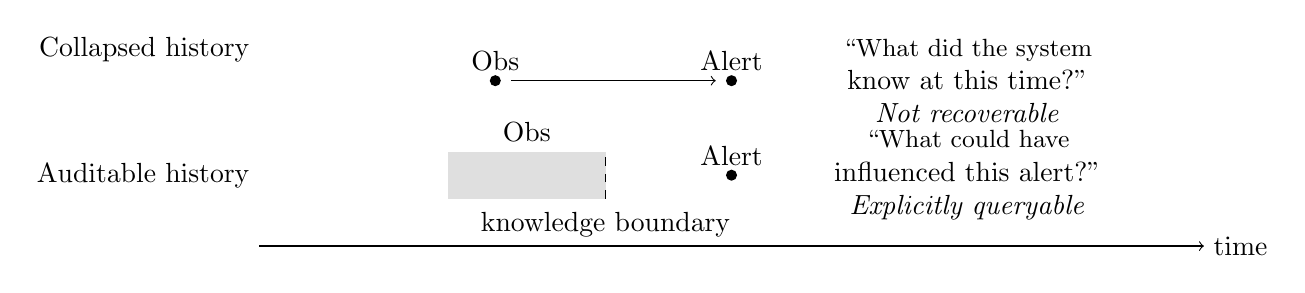
\begin{tikzpicture}[x=1cm,y=1cm]

% Time axis
\draw[->] (0,0) -- (12,0) node[right]{time};

% Labels
\node[anchor=east] at (0,2.5) {Collapsed history};
\node[anchor=east] at (0,0.9) {Auditable history};

% ---- Collapsed history ----
% Events
\fill (3,2.1) circle (2pt);
\node[above] at (3,2.1) {Obs};

\fill (6,2.1) circle (2pt);
\node[above] at (6,2.1) {Alert};

% Arrow
\draw[->] (3.2,2.1) -- (5.8,2.1);

% Annotation
\node[align=center] at (9,2.1)
  {\small ``What did the system\\know at this time?''\\\textit{Not recoverable}};

% ---- Auditable history ----
% Observation interval
\draw[fill=gray!25,draw=none] (2.4,0.6) rectangle (4.4,1.2);
\node[above] at (3.4,1.2) {Obs};

% Alert point
\fill (6,0.9) circle (2pt);
\node[above] at (6,0.9) {Alert};

% Knowledge window
\draw[dashed] (4.4,0.6) -- (4.4,1.2);
\node[below] at (4.4,0.55) {knowledge boundary};

% Annotation
\node[align=center] at (9,0.9)
  {\small ``What could have\\influenced this alert?''\\\textit{Explicitly queryable}};

\end{tikzpicture}
}
\caption{Auditability under collapsed versus propagated time. \conceptual\; When timestamps are rewritten or normalised (top), historical system state cannot be reconstructed; when temporal uncertainty is preserved (bottom), the system retains an explicit boundary between what was known and what was not, enabling post-hoc audit, explanation, and governance.}
\end{figure}

\end{document}